\section{Training Neural Networks with \textbf{\textit{clDice}}}
In the previous section we provided general theoretic guarantees how \textit{clDice} has topology preserving properties. The following chapter shows how we applied our theory to efficiently train topology preserving networks using the \textit{clDice} formulation. \footnote{\url{https://github.com/jocpae/clDice}}

\begin{figure*}[]
\begin{center}
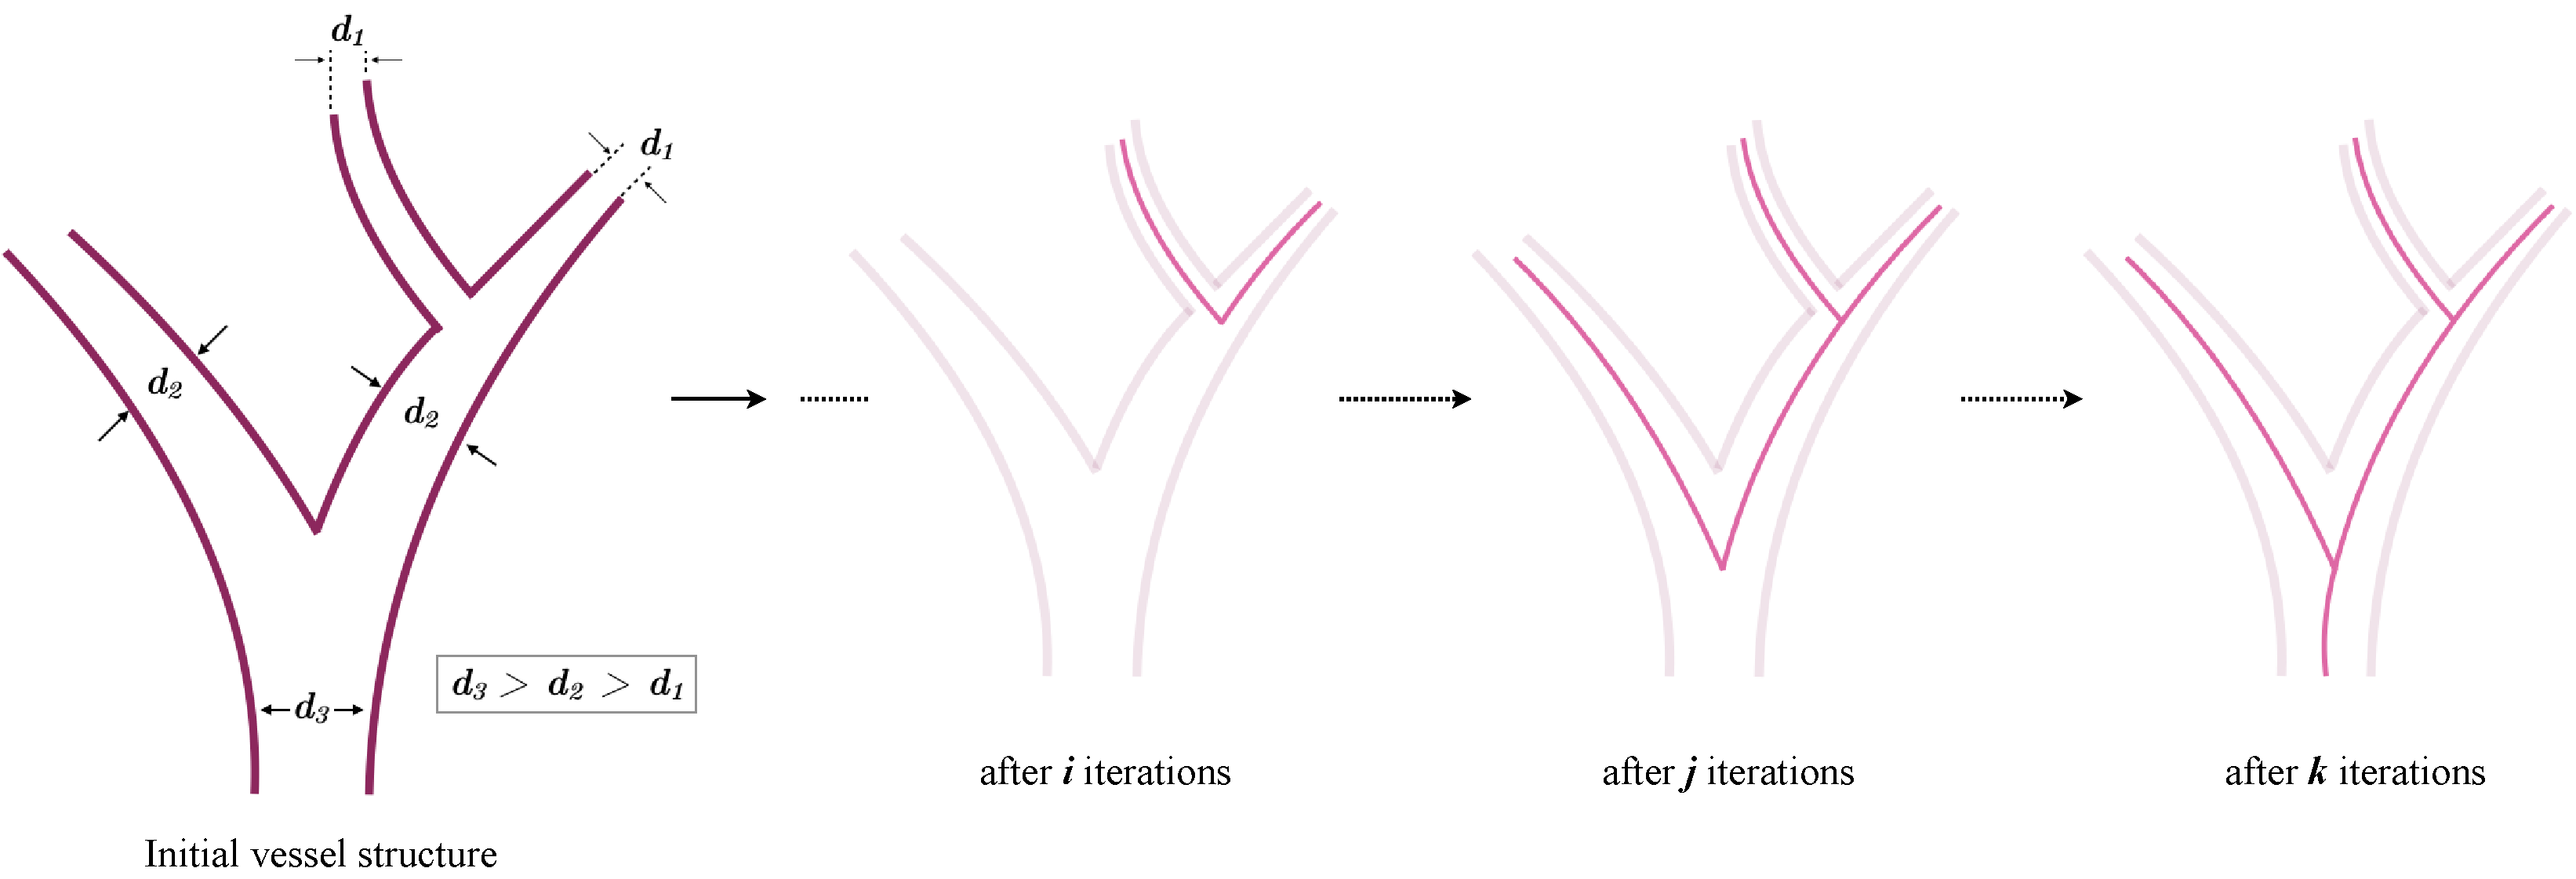
\includegraphics[width=0.9\linewidth]{figs/sequence_toy.pdf}
\end{center}
\caption{ Based on the initial vessel structure (purple), sequential bagging of skeleton voxels (red) via iterative skeletonization leads to a complete skeletonization, where $d$ denotes the diameter and  $k>j>i$ iterations.}
\label{seq_skel}
\vspace{-1em}
\end{figure*}

\subsection{\textbf{\textit{Soft-clDice}} using \textbf{\textit{Soft-skeletonization}}:}
Extracting accurate skeletons is essential to our method. For this task, a multitude of approaches has been proposed. However, most of them are not fully differentiable and therefore unsuited to be used in a loss function. Popular approaches use the Euclidean distance transform or utilize repeated morphological thinning. Euclidean distance transform has been used on multiple occasions \cite{shih1995skeletonization,wright1995skeletonization}, but remains a discrete operation and, to the best of our knowledge, an end-to-end differentiable approximation remains to be developed, preventing the use in a loss function for training neural networks.
On the contrary, morphological thinning is a sequence of dilation and erosion operations [c.f. Fig. \ref{seq_skel}].

\begin{figure}[t!]
\begin{minipage}{0.45\textwidth}
\removelatexerror
    \begin{algorithm*}[H]
        \caption{\textit{soft-skeleton}}
        \label{algorithm-1}
        \SetKwInOut{Input}{Input}
        \Input{$I,k$}
        \begin{algorithmic}
        \State $I' \gets \textit{maxpool}(\textit{minpool}(I))$
        \State $S \gets \textit{ReLU}(I-I')$
        \end{algorithmic}
        \For{$i\gets0$ \KwTo $k$}{
            $I \gets  \textit{minpool}(I)$\\
            $I' \gets \textit{maxpool}(\textit{minpool}(I))$\\
            $S \gets S+(1-S)\circ \textit{ReLU}(I-I')$
        }
        \SetKwInOut{Output}{Output}
        \Output{$S$}
    \end{algorithm*}
    \begin{algorithm*}[H]
        \caption{\textit{soft-clDice}}
        \label{algorithm-2}
        \SetKwInOut{Input}{Input}
        \Input{$V_P,V_L$}
        \begin{algorithmic}
            \State $S_P \gets \mbox{\textit{soft-skeleton}}(V_P)$
            \State $S_L \gets \mbox{\textit{soft-skeleton}}(V_L)$
            \State $\textit{Tprec}(S_P, V_L) \gets \frac{|S_P \circ V_L|+\epsilon}{|S_P|+\epsilon}$
            \State $\textit{Tsens}(S_L, V_P) \gets \frac{|S_L \circ V_P|+\epsilon}{|S_L|+\epsilon}$
            \State $\textit{clDice} \gets$ \par
            $2 \times \frac{ \textit{Tprec}(S_P, V_L)\times \textit{Tsens}(S_L, V_P)}{\textit{Tprec}(S_P, V_L)+ \textit{Tsens}(S_L, V_P)}$
        \end{algorithmic}
        \vspace{0.2cm}
        \SetKwInOut{Output}{Output}
        \Output{$clDice$}
    \end{algorithm*}
\end{minipage}    
 \caption{ \textbf{Algorithm \ref{algorithm-1}} calculates the proposed \textit{soft-skeleton}, here $I$ is the mask to be \textit{soft-skeletonized} and $k$ is the number of iterations for skeletonization. \textbf{Algorithm \ref{algorithm-2}}, calculates the \textit{soft-clDice} loss, where $V_P$ is a real-valued probabilistic prediction from a segmentation network and $V_L$ is the true mask. We denote Hadamard product using $\circ$.}
 \vspace{-1.5em}
\end{figure}
Importantly, thinning using morphological operations (skeletonization) on curvilinear structures can be topology-preserving \cite{palagyi20023}. Min- and max filters are commonly used as the grey-scale alternative of morphological dilation and erosion. Motivated by this, we propose `soft-skeletonization', where an iterative min- and max-pooling is applied as a proxy for morphological erosion and dilation. The Algorithm \ref{algorithm-1} describes the iterative processes involved in its computation. The hyper-parameter $k$ involved in its computation represents the iterations and has to be greater than or equal to the maximum observed radius. In our experiments, this parameter depends on the dataset. For example, it is  $k=5...25$ in our experiments, matching the pixel radius of the largest observed tubular structures. Choosing a larger $k$ does not reduce performance but increases computation time. On the other hand, a too low $k$ leads to incomplete skeletonization. 

% \textbf{This skeleton-approximation is not guaranteed to be fully topology preserving; however, a better dif-
% ferentiable skeletonization can only improve performance, which we reserve for future research.}

In Figure \ref{seq_skel}, the successive steps of our skeletonization are intuitively represented. In the early iterations, the structures with a small radius are skeletonized and preserved until the later iterations when the thicker structures become skeletonized. This enables the extraction of a parameter-free, morphologically motivated soft-skeleton. The aforementioned soft-skeletonization enables us to use \textit{clDice} as a fully differentiable, real-valued, optimizable measure. The Algorithm \ref{algorithm-2} describes its implementation. We refer to this as the \textit{soft-clDice}.

For a single connected foreground component and in the absence of knots, the homotopy type is specified by the number of linked loops. Hence, if the reference and the predicted volumes are not homotopy equivalent, they do not have pairwise linked loops. To include these missing loops or exclude the extra loops, one has to add or discard deformation retracted skeleta of the solid foreground. This implies adding \textit{new correctly predicted voxels}. In contrast to other volumetric losses such as Dice, cross-entropy, etc., \textit{clDice} only considers the deformation-retracted graphs of the solid foreground structure. Thus, we claim that \textit{clDice} requires the least amount of \textit{new correctly predicted voxels} to guarantee the homotopy equivalence. Along these lines, Dice or cross-entropy can only guarantee homotopy equivalence if every single voxel is segmented correctly. On the other hand, \textit{clDice} can guarantee homotopy equivalence for a broader combinations of connected-voxels. Intuitively, this is a very much desirable property as it makes \textit{clDice} robust towards outliers and noisy segmentation labels.


\subsection{Cost Function}
Since our objective here is to preserve topology while achieving accurate segmentations, and not to learn skeleta, we combine our proposed \textit{soft-clDice} with \textit{soft-Dice} in the following manner: 
\begin{equation}
\mathcal{L}_{c} = (1-\alpha)(1-\mbox{\textit{soft\textbf{Dice}})}+\alpha(1-\mbox{\textit{soft\textbf{clDice}}) }
\label{eq3}
\end{equation}
where $\alpha \in [0,0.5]$. In stark contrast to previous works, where segmentation and centerline prediction has been learned jointly as multi-task learning \cite{uslu2018multi,tetteh2018deepvesselnet}, we are not interested in learning the centerline. We are interested in learning a topology-preserving segmentation. Therefore, we restrict our experimental choice of alpha to $\alpha \in [0,0.5]$.
We test \textit{clDice} on two state-of-the-art network architectures: i) a 2D and 3D U-Net\cite{ronneberger2015u,cciccek20163d}, and ii) a 2D and 3D fully connected networks (FCN) \cite{tetteh2018deepvesselnet,gerlRSOM}. As baselines, we use the same architectures trained using \textit{soft-Dice} \cite{milletari2016v,sudre2017generalised}.

\subsection{Adaption for Highly Imbalanced Data}
Our theory  (Section \ref{sec:proof}), describes a two-class problem where \textit{clDice} should be computed on both the foreground and the background channels. In our experiments, we show that for complex and highly imbalanced dataset it is sufficient to calculate the \textbf{clDice} loss on the underrepresented foreground class. We attribute this to the distinct properties of tubularness, sparsity of foreground and the lack of cavities (Betti number 2) in our data. An intuitive interpretation how these assumptions are valid in terms of digital topology can be found in the supplementary material.

%3D vascular or road structures, we approximate our theoryHowever, in practice, this is hindered by an imbalance in the foreground and background classes (e.g. in vessel and road datasets).
%The class imbalance would substantially enhance the computational complexity in calculating the skeletons on the majority class (typically the background class). Thus, we calculate the \textit{clDice} only on the foreground. 

\section{Experiments}
\subsection{Datasets} 
We employ five public datasets for validating \textit{clDice} and \textit{soft-clDice} as a measure and an objective function, respectively. In 2D, we evaluate on the DRIVE retina dataset \cite{staal2004ridge}, the Massachusetts Roads dataset \cite{MnihThesis} and the CREMI neuron dataset \cite{Funke_2019}. In 3D, a synthetic vessel dataset with an added Gaussian noise term \cite{schneider2012tissue} and the Vessap dataset of multi-channel volumetric scans of brain vessels is used \cite{todorov2019automated,paetzold2019transfer}. For the Vessap dataset we train different models for one and two input channels. 
%\footnote{ \url{https://drive.grand-challenge.org/}}
%\footnote{ \url{https://www.cs.toronto.edu/~vmnih/data/}}
%
%(voxel size: ($3 \mu m^3$)), which were obtained using light-sheet microscopy of tissue cleared Murine brains, and made publicly available in \footnote{ \url{http://discotechnologies.org/VesSAP/}}.
For all of the datasets, we perform three fold cross-validation and test on held-out, large, and highly-variant test sets. Details concerning the experimental setup can be found in the supplementary.
\subsection{Evaluation Metrics}
We compare the performance of various experimental setups using three types of metrics: volumetric, topology-based, and graph-based. 
\begin{enumerate}[itemsep=0pt,parsep=0pt]
    \item Volumetric: We compute volumetric scores such as Dice coefficient, Accuracy, and the proposed \textit{clDice}.
    \item Topology-based: We calculate the mean of absolute Betti Errors for the Betti Numbers $\beta_0$ and $\beta_1$ and the mean absolute error of Euler characteristic, $\chi = V-E+F$, where $V, E, \mbox{ and } F$ denotes number of vertices, edges, and faces.
    \item Graph-based: we extract random patch-wise graphs for the 2D/3D images. We uniformly sample fixed number of points from the graph and compute the StreetmoverDistance (SMD) \cite{belli2019image}. SMD captures a Wasserstein distance between two graphs. Additionally we compute the F1 score of junction-based metric \cite{citrarotowards}.
\end{enumerate}

\begin{table*}[!ht]
\caption{ Quantitative experimental results for the Massachusetts road dataset (Roads), the CREMI dataset, the DRIVE retina dataset and the Vessap dataset (3D). Bold numbers indicate the best performance. The performance according to the \textit{clDice} measure is highlighted in rose. For all experiments we observe that using \textit{soft-clDice} in $\mathcal{L}_{c}$ results in improved scores compared to \emph{soft-Dice}. This improvement holds for almost $\alpha > 0$; $\alpha$ can be interpreted as a dataset specific hyper-parameter.}

\centering
\label{final_table}
\footnotesize
\begin{tabular}{lll|c c>{\columncolor{red!20}} c|cc|ccc}

\hline\hline
%%%%%%%%%%%%% ------------ ROADS
Dataset & Network & Loss & Dice & Accuracy & \textit{clDice} & $\beta_0$ Error &  $\beta_1$ Error  & SMD \cite{belli2019image} &  $\chi_{error}$ & Opt-J F1 \cite{citrarotowards}\\
\hline\hline
\multirow{13}{*}{Roads}    & \multirow{2}{*}{FCN} &  \textit{soft-dice} & 64.84 & 95.16 & 70.79 & 1.474 & 1.408 & 0.1216 & 2.634 & 0.766\\ \cdashline{3-11}[2pt/2pt]
&   & $\mathcal{L}_{c}, \alpha = 0.1$     & 66.52 & 95.70 & 74.80 & 0.987 & 1.227 & 0.1002 & 2.625 & 0.768\\
&   & $\mathcal{L}_{c}, \alpha = 0.2$     & \textbf{67.42}& \textbf{95.80} & 76.25 & \textbf{0.920} & 1.280 & \textbf{0.0954} & 2.526 & 0.770\\
&   & $\mathcal{L}_{c}, \alpha = 0.3$     & 65.90 & 95.35 & 74.86 & 0.974 & 1.197 & 0.1003 & 2.448 & 0.775\\
&   & $\mathcal{L}_{c}, \alpha = 0.4$     & 67.18 & 95.46 & \textbf{76.92} & 0.934 & \textbf{1.092} & 0.0991 & \textbf{2.183} & \textbf{0.803}\\
&   & $\mathcal{L}_{c}, \alpha = 0.5$     & 65.77 & 95.09 & 75.22 & 0.947 & 1.184 & 0.0991 & 2.361 & 0.782\\
  \cline{2-11}

& \multirow{6}{*}{U-NET} & \textit{soft-dice} & 76.23 & 96.75 & 86.83 & 0.491 & 1.256 & 0.0589 & 1.120 & 0.881\\ \cdashline{3-11}[2pt/2pt]
&  & $\mathcal{L}_{c}, \alpha = 0.1$  & \textbf{76.66} & \textbf{96.77} & 87.35 & 0.359 & \textbf{0.938} & 0.0457 & 0.980 & 0.878\\
&  & $\mathcal{L}_{c}, \alpha = 0.2$  & 76.25 & 96.76 & 87.29 & \textbf{0.312} & 1.031 & \textbf{0.0415} & 0.865 & 0.900\\
&  & $\mathcal{L}_{c}, \alpha = 0.3$  & 74.85 & 96.57 & 86.10 & 0.322 & 1.062 & 0.0504 & 0.827 & 0.913\\
&  & $\mathcal{L}_{c}, \alpha = 0.4$  & 75.38 & 96.60 & 86.16 & 0.344 & 1.016 & 0.0483 & \textbf{0.755} & \textbf{0.916}\\
&  & $\mathcal{L}_{c}, \alpha = 0.5$  & 76.45 & 96.64 & \textbf{88.17} & 0.375 & 0.953 & 0.0527 & 1.080 & 0.894\\\cline{2-11}
& Mosinska et al. & \cite{mosinska2018beyond,hu2019topology} & - & 97.54 & - & - & 2.781 & - & - & -\\
& Hu et al. & \cite{hu2019topology} & - & 97.28 & - & - & 1.275 & - & - & -\\
%%%%%%%%%%%%%%%%% ------------    CREMI 
\hline\hline
\multirow{9}{*}{CREMI}   
& \multirow{6}{*}{U-NET} & \textit{soft-dice} & 91.54 & 97.11 & 95.86 & 0.259 & 0.657 & 0.0461 & 1.087 & 0.904\\ \cdashline{3-11}[2pt/2pt]
%&  & $\mathcal{L}_{c}, \alpha = 0.001$& 91.681 & 95.885 & 97.148 & & & &\\
%&  & $\mathcal{L}_{c}, \alpha = 0.01$ & 91.734 & 96.013 & 97.204 & & & &\\
&  & $\mathcal{L}_{c}, \alpha = 0.1$  & 91.76 & \textbf{97.21} & 96.05 & 0.222 & 0.556 & \textbf{0.0395} & 1.000 & 0.900\\
&  & $\mathcal{L}_{c}, \alpha = 0.2$  & 91.66 & 97.15 & 96.01 & 0.231 & 0.630 & 0.0419 & 0.991 & 0.902\\
&  & $\mathcal{L}_{c}, \alpha = 0.3$  & \textbf{91.78} & 97.18 & \textbf{96.21} & \textbf{0.204} & \textbf{0.537} & 0.0437 & \textbf{0.919} & \textbf{0.913}\\
&  & $\mathcal{L}_{c}, \alpha = 0.4$  & 91.56 & 97.12 & 96.09 & 0.250 & 0.630 & 0.0444 & 0.995 & 0.902\\
&  & $\mathcal{L}_{c}, \alpha = 0.5$  & 91.66 & 97.16 & 96.16 & 0.231 & 0.620 & 0.0455 & 0.991 & 0.907\\\cline{2-11}
& Mosinska et al. & \cite{mosinska2018beyond,hu2019topology} & 82.30 & 94.67 & - & - & 1.973 & - & - & -\\
& Hu et al. & \cite{hu2019topology} & - & 94.56 & - & - & 1.113 & - & - & -\\
\hline\hline                              
%%%%%%%%%%%%%%%%% ------------    DRIVE 
\multirow{10}{*}{DRIVE retina~}& \multirow{6}{*}{FCN} & \textit{soft-Dice} & 78.23  & 96.27 & 78.02  & 2.187 & 1.860 & 0.0429 & 3.275 & 0.773\\ \cdashline{3-11}[2pt/2pt]
&   & $\mathcal{L}_{c}, \alpha = 0.1$     & 78.36 & 96.25 & 79.02 & 2.100 & 1.610 & 0.0393 & 3.203 & 0.777\\
&   & $\mathcal{L}_{c}, \alpha = 0.2$     & \textbf{78.75} & 96.29 & 80.22 & 1.892 & 1.382 & 0.0383 & 2.895 & 0.793\\
&   & $\mathcal{L}_{c}, \alpha = 0.3$     & 78.29 & 96.20 & 80.28 & 1.888 & \textbf{1.332} & \textbf{0.0318} & 2.918 & \textbf{0.798}\\
&   & $\mathcal{L}_{c}, \alpha = 0.4$     & 78.00 & 96.11 & 80.43 & 2.036 & 1.602 & 0.0423 & 3.141 & 0.764\\
&   & $\mathcal{L}_{c}, \alpha = 0.5$     & 77.76 & 96.04 & \textbf{80.95} & \textbf{1.836} & 1.408 & 0.0394 & \textbf{2.848} & 0.794\\\cline{2-11}
 & \multirow{2}{*}{U-Net} & \textit{soft-Dice} & 74.25 & 95.63 & 75.71 & 1.745 & 1.455 & 0.0649 & 2.997 & 0.760\\
&    & $\mathcal{L}_{c}, \alpha = 0.5$   & \textbf{75.21} & \textbf{95.82} & \textbf{76.86} & \textbf{1.538} & \textbf{1.389} & \textbf{0.0586} & \textbf{2.737} & \textbf{0.767}\\\cline{2-11}
& Mosinska et al. & \cite{mosinska2018beyond,hu2019topology} & - & 95.43 & - & - & 2.784 & - & - & -\\
& Hu et al. & \cite{hu2019topology} & - & 95.21 & - & - & 1.076 & - & - & -\\
\hline\hline
%%%%%%%%%%%%%%%%%% ------- 3D DATA

\multirow{16}{*}{Vessap data}    & \multirow{2}{*}{FCN, 1 ch} &  \textit{soft-dice}  & 85.21 & \textbf{96.03} & 90.88 & 3.385 & 4.458 & 0.00459 & 5.850 & 0.862\\ 
  & &$\mathcal{L}_{c}, \alpha = 0.5$  & \textbf{85.44} & 95.91 & \textbf{91.32} & \textbf{2.292} & \textbf{3.677} & \textbf{0.00417} & \textbf{5.620} & \textbf{0.864}\\
  \cline{2-11}
  
& \multirow{6}{*}{FCN, 2 ch} & \textit{soft-dice} & 85.31 & 95.82 & 90.10 & 2.833 & 4.771 & 0.00629 & 6.080 & 0.849\\\cdashline{3-11}[2pt/2pt]
&  & $\mathcal{L}_{c}, \alpha = 0.1$  & 85.96 & 95.99 & 91.02 & 2.896 & \textbf{4.156} & 0.00447 & 5.980 & 0.860\\
&  & $\mathcal{L}_{c}, \alpha = 0.2$  & \textbf{86.45} & \textbf{96.11} & 91.22 & 2.656 & 4.385 & 0.00466 & 5.530 & 0.869\\
&  & $\mathcal{L}_{c}, \alpha = 0.3$  & 85.72 & 95.93 & 91.20 & 2.719 & 4.469 & \textbf{0.00423} & 5.470 & 0.866\\
&  & $\mathcal{L}_{c}, \alpha = 0.4$  & 85.65 & 95.95 & \textbf{91.65} & 2.719 & 4.469 & \textbf{0.00423} & 5.670 & 0.869\\
&  & $\mathcal{L}_{c}, \alpha = 0.5$  & 85.28 & 95.76 & 91.22 & \textbf{2.615} & 4.615 & 0.00433 & \textbf{5.320} & \textbf{0.870}\\
 \cline{2-11}
& \multirow{2}{*}{U-Net, 1 ch} & \textit{soft-dice} & 87.46 & 96.35 & 91.18 & 3.094 & 5.042 & 0.00549 & 5.300 & 0.863\\ 
&  & $\mathcal{L}_{c}, \alpha = 0.5$ & \textbf{87.82} & \textbf{96.52} & \textbf{93.03} & \textbf{2.656} & \textbf{4.615} & \textbf{0.00533} & \textbf{4.910} & \textbf{0.872}\\
    \cline{2-11}
& \multirow{6}{*}{U-Net, 2 ch} & \textit{soft-dice} & 87.98 & 96.56 & 90.16 & 2.344 & 4.323 & 0.00507 & 5.550 & 0.855\\ \cdashline{3-11}[2pt/2pt]
&  & $\mathcal{L}_{c}, \alpha = 0.1$ & 88.13 & 96.59 & 91.12 & 2.302 & 4.490 & 0.00465 & 5.180 & \textbf{0.872}\\
&  & $\mathcal{L}_{c}, \alpha = 0.2$ & 87.96 & 96.74 & 92.52 & 2.208 & \textbf{3.979} & 0.00342 & \textbf{4.830} & 0.861\\
&  & $\mathcal{L}_{c}, \alpha = 0.3$ & 87.70 & 96.71 & 92.56 & \textbf{2.115} & 4.521 & \textbf{0.00309} & 5.260 & 0.858\\
&  & $\mathcal{L}_{c}, \alpha = 0.4$ & \textbf{88.57} & \textbf{96.87} & \textbf{93.25} & 2.281 & 4.302 & 0.00327 & 5.370 & 0.868
\\
&  & $\mathcal{L}_{c}, \alpha = 0.5$ & 88.14 & 96.74 & 92.75 & 2.135 & 4.125 & 0.00328 & 5.390 & 0.864\\
\hline\hline

\end{tabular}
\vspace{-1.5em}
\end{table*}


\subsection{Results and Discussion}
We trained two segmentation architectures, a U-Net and an FCN, for the various loss functions in our experimental setup. As a baseline, we trained the networks using \textit{soft-dice} and compared it with the ones trained using the proposed loss (Eq.~\ref{eq3}), by varying $\alpha$ from (0.1 to 0.5).
\vspace{0.15cm}

\noindent\textbf{Quantitative:} We observe that including \textit{soft-clDice} in any  proportion ($\alpha>0$) leads to improved topological, volumetric and graph similarity for all 2D and 3D datasets, see Table \ref{final_table}. We conclude that $\alpha$ can be interpreted as a hyper parameter which can be tuned \emph{per-dataset}. Intuitively, increasing the  $\alpha$ improves the \textit{clDice} measure for most experiments. Most often, \textit{clDice} is high or highest when the graph and topology based measures are high or highest, particularly the $\beta_1$ Error,  Streetmover distance and  Opt-J F1 score; quantitatively indicating that topological properties are indeed represented in the \textit{clDice} measure.

In spite of not optimizing for a high \textit{soft-clDice} on the background class, all of our networks converge to superior segmentation results. This not only reinforces our assumptions on dataset-specific necessary conditions but also validates the practical applicability of our loss. 
Our findings hold for the different network architectures, for 2D or 3D, and for tubular or curvilinear structures, strongly indicating its generalizability to analogous binary segmentation tasks.\\

Observe that CREMI and the synthetic vessel dataset (see Supplementary material) appear to have the smallest increase in scores over the baseline. We attribute this to them being the least complex datasets in the collection, with CREMI having an almost uniform thickness of radii and the synthetic data having a high signal-to-noise ratio and insignificant illumination variation. 
More importantly, we observe larger improvements for all measures in case of the more complex Vessap and Roads data see Figure \ref{road_result}.
In direct comparison to performance measures reported in two recent publications by Hu et al. and Mosinska et al. \cite{hu2019topology,mosinska2018beyond}, we find that our approach is on par or better in terms of Accuracy and Betti Error for the Roads and CREMI dataset. It is important to note that we used a smaller subset of training data for the Road dataset compared to both while using the same test set. 

Hu et al. reported a Betti error for the DRIVE data, which exceeds ours; however, it is important to consider that their approach explicitly minimizes the mismatch of the persistence diagram, which has significantly higher computational complexity during training, see the section below.
We find that our proposed loss performs superior to the baseline in almost every scenario. The improvement appears to be pronounced when evaluating the highly relevant graph and topology based measures, including the recently introduced OPT-Junction F1 by Citraro et al. \cite{citrarotowards}.  Our results are consistent across different network architectures, indicating that \textit{soft-clDice} can be deployed to any network architecture.

\noindent\textbf{Qualitative: }In Figure \ref{road_result}, typical results for our datasets are depicted. Our networks trained on the proposed loss term recover connections, which were false negatives when trained with the soft-Dice loss. These missed connections appear to be particularly frequent in the complex road and DRIVE dataset. For the CREMI dataset, we observe these situations less frequently, which is in line with the very high quantitative scores on the CREMI data. 
Interestingly, in the real 3D vessel dataset, the soft-Dice loss oversegments vessels, leading to false positive connections. This is not the case when using our proposed loss function, which we attribute to its topology-preserving nature. Additional qualitative results can be inspected in the supplementary.\\

\noindent\textbf{Computational Efficiency: }Naturally, inference times of CNNs with the same architecture but different training losses are identical. However, during training, our soft-skeleton algorithm requires $O(kn^2)$ complexity for an $n\times n$ 2D image where $k$ is the number of iterations. As a comparison, \cite{hu2019topology} needs $O(c^2mlog(m))$ (see \cite{han2003topology}) complexity to compute the 1d persistent homology where $d$ is the number of points with zero gradients in the prediction and $m$ is the number of simplices. Roughly, $c$ is proportional to $n^2$, and $m$ is of $O(n^2)$ for a 2D Euclidean grid. Thus, the worst complexity of \cite{hu2019topology} is $O(n^6log(n))$. 
Additionally, their approach requires an $O(clog(c))$ complexity to find an optimal matching of the birth-death pairs. We note that the total run-time overhead for soft-clDice compared to soft-Dice is marginal, i.e., for batch-size of 4 and 1024x1024 image resolution, the former takes 1.35s while the latter takes 1.24s on average ($<$10\% increase) on an RTX-8000.\\

\noindent\textbf{Future Work: }Although our proposed soft-skeleton approximation works well in practice, a better differentiable skeletonization can only improve performance, which we reserve for future research. Any such skeletonization can be readily plugged into our approach. Furthermore, theoretical and experimental multi-class studies would sensibly extend our study.

\section{Conclusive Remarks}
We introduce \textit{clDice}, a novel topology-preserving similarity measure for tubular structure segmentation. Importantly, we present a theoretical guarantee that \textit{clDice} enforces topology preservation up to homotopy equivalence. Next, we use a differentiable version of the \textit{clDice}, \textit{soft-clDice}, in a loss function, to train state-of-the-art 2D and 3D neural networks. We use \textit{clDice} to benchmark segmentation quality from a topology-preserving perspective along with multiple volumetric, topological, and graph-based measures.  We find that training on \textit{soft-clDice} leads to segmentations with more accurate connectivity information, better graph-similarity, better Euler characteristics, and improved Dice and Accuracy. Our \textit{soft-clDice} is computationally efficient and can be readily deployed to any other deep learning-based segmentation tasks such as neuron segmentation in biomedical imaging, crack detection in industrial quality control, or remote sensing.\\

\noindent \textbf{Acknowledgement: } J. C. Paetzold. and S. Shit. are supported by the GCB and Translatum, TU Munich. S.Shit., A. Zhylka. and I. Ezhov. are supported by TRABIT (EU Grant: 765148). We thank Ali Ertuerk, Mihail I. Todorov, Nils Börner and Giles Tetteh.

% Suprosanna Shit, Andrey Zhylka and Ivan Ezhov are supported by the Translational Brain Imaging Training Network(TRABIT) under the European Union's `Horizon 2020' research \& innovation program (Grant agreement ID: 765148). With the support of the Technical University of Munich – Institute for Advanced Study, funded by the German Excellence Initiative.


%%%%%%%%%%%%%%%%55-------------------%%%%%%%%%%%%%%%%%%%%%%%%%%%%
\begin{figure}[ht!]

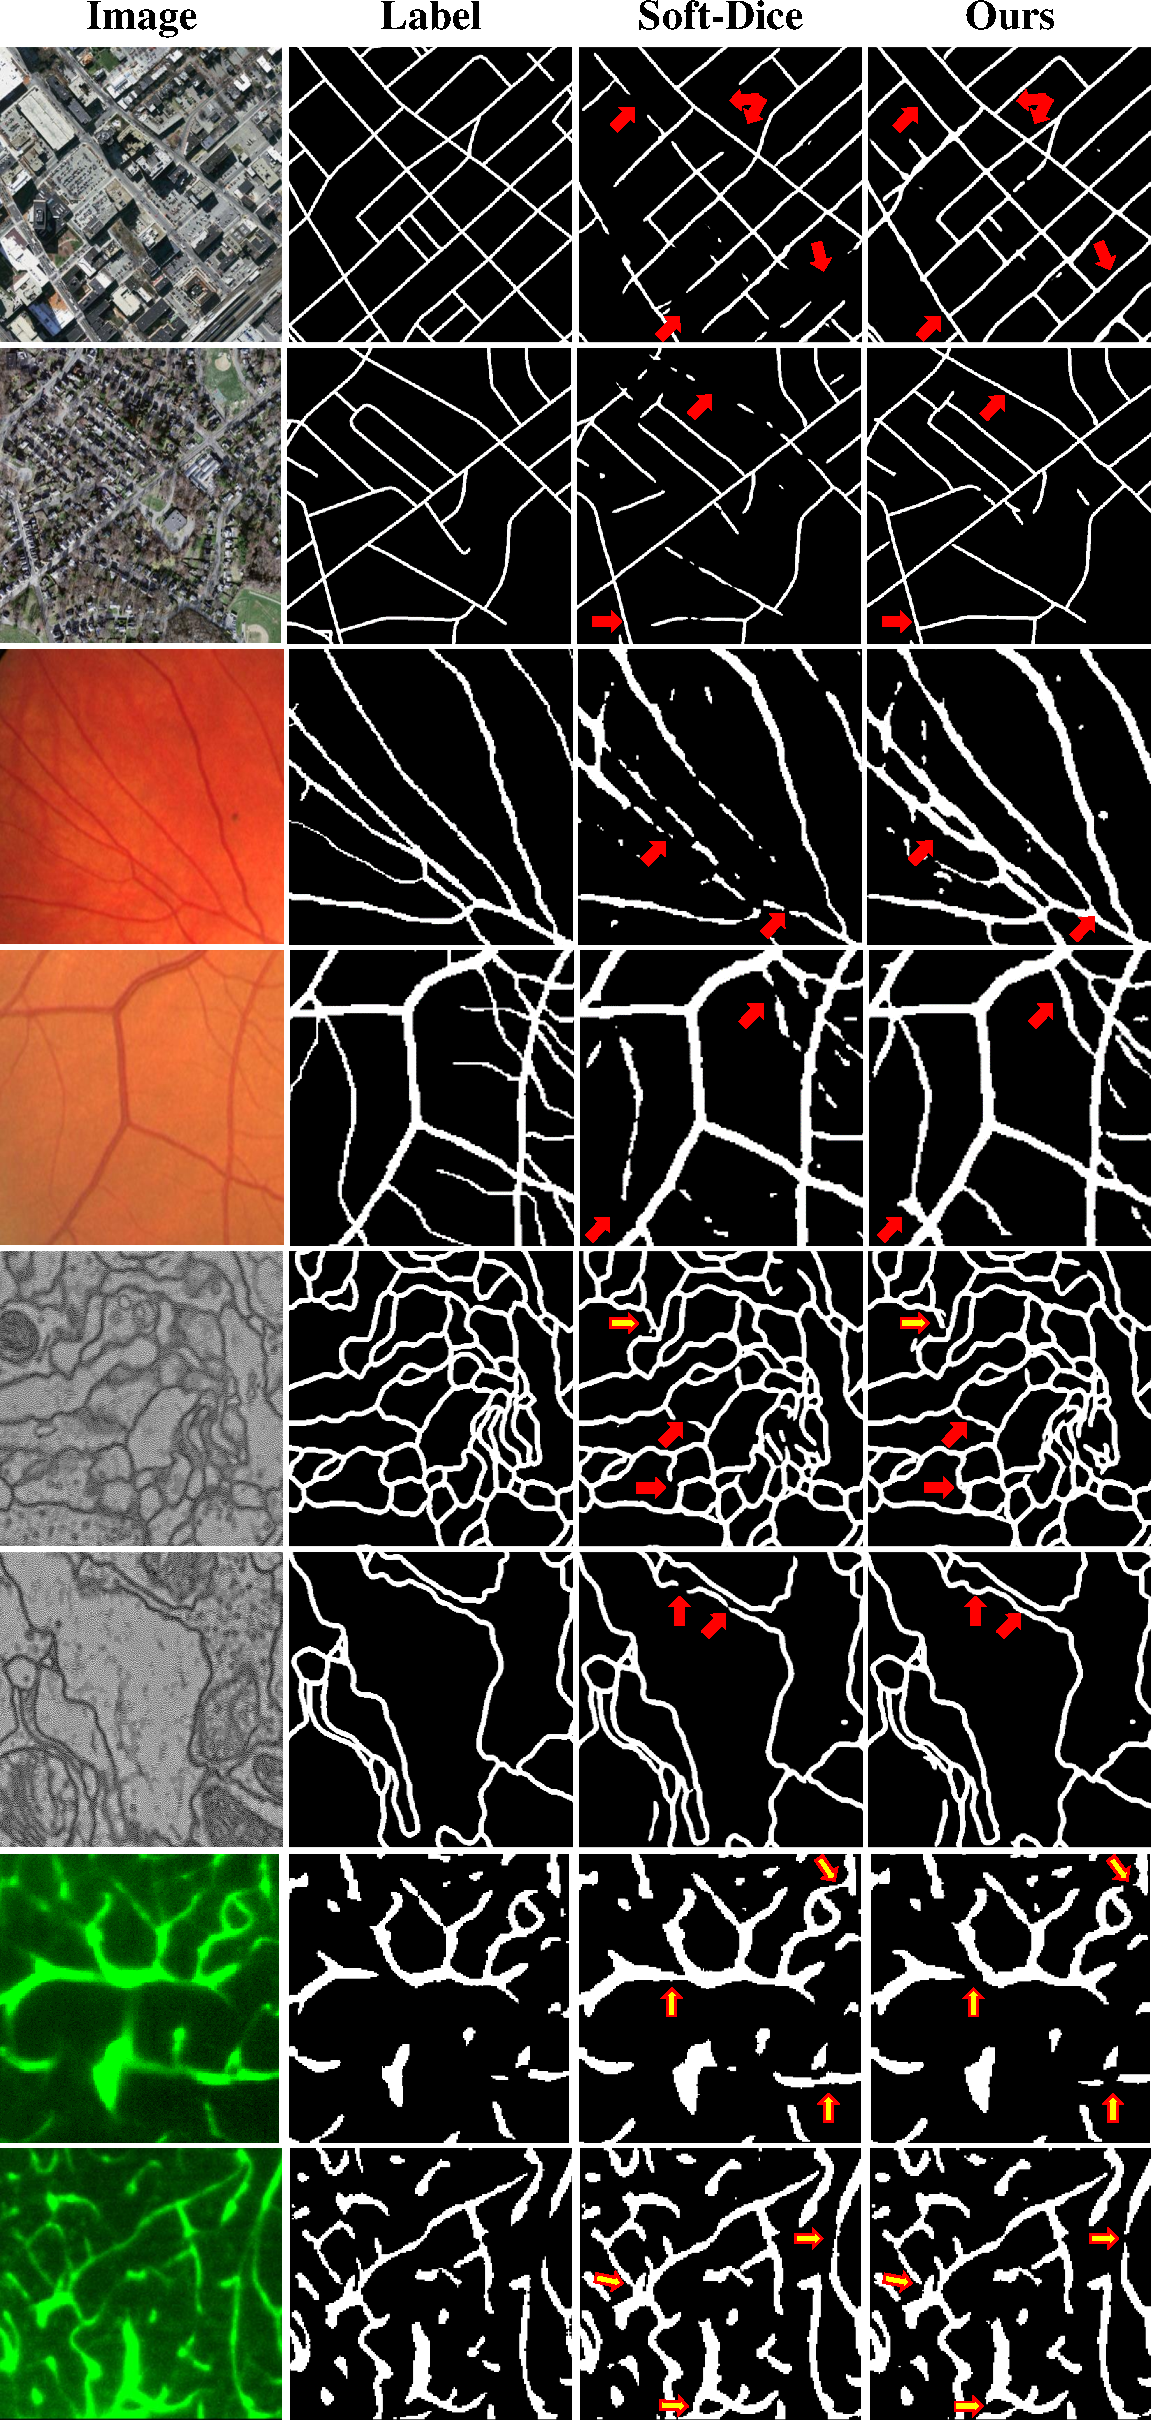
\includegraphics[width=0.98\linewidth]{figs/clDice_qualitative_results.pdf}

\caption{Qualitative results: from top to bottom we show two rows of results for: the Massachusetts road dataset, the DRIVE retina dataset, the CREMI neuron data and 2D slices from the 3D Vessap dataset. From left to right, the real image, the label, the prediction using soft-Dice and the U-Net predictions using $\mathcal{L}_c (\alpha=0.5)$ are shown, respectively. The images indicate that \textit{clDice} segments road, retina vessel connections and neuron connections which the soft-Dice loss misses, but also does not segment false-positive vessels in 3D. Some, but not all, missed connections are indicated with solid red arrows, false positives are indicated with red-yellow arrows. More qualitative results can be found in the Supplementary material.}
\label{road_result}
\end{figure}
%%%%%%%%%%%%%%%%-------------------%%%%%%%%%%%%%%%%%%%%%%%%%%%%